\section{Database Design}
\label{section:databaseDesign}

To store the raw data, a method that provides reliability, scalability, ease of maintenance and good performance is required. The easiest solution would be to store all of the raw data in plain text files or as comma separated values (CSV) files, nevertheless this approach is neither scalable nor good for performance, furthermore, there is no straightforward way to ensure the data consistency. Instead, a database design is proposed here, this design overcomes most of the drawbacks exhibited by a plain text file approach. 

Before getting into the details of the database design it is important to remark the concept of a \textit{primary key} in the context of databases. Within an entity (table) in a database a specific instance of such entity can be uniquely identified by means of the so called primary key. It is also important to mention that for the design of the database we have considered two kinds of mechanical components in the \gls{hvac} network. The so called basic components are the smaller ``logical'' building blocks for the \gls{hvac} system; fans, dampers, cooling and heating coils (generalized here as heat exchanger coils), filters and VFDs belong to this category. The major components are the more complex and larger pieces of equipment of the \gls{hvac} system, they are made up of a number of the basic components that work together to achieve a specific goal (like controlling the amount of airflow that is distributed to a certain area in the case of \glspl{vav}).

Some further considerations need to be taken for the development of the database that will store the sensor readings, the most relevant ones are listed next

\begin{itemize}
\item The data must allow the storage of the readings as time-series.
\item The database must reflect the general layout of the \gls{hvac} system.
\item The database should help pinpoint the location of the faults.
\item The database should allow the aggregation of other sensor readings easily.
\item Each one of the component in the \gls{hvac} network must be easily identifiable.
\end{itemize}

To comply we the above requirements the following database was designed

\begin{figure}[H]
	\centering
  	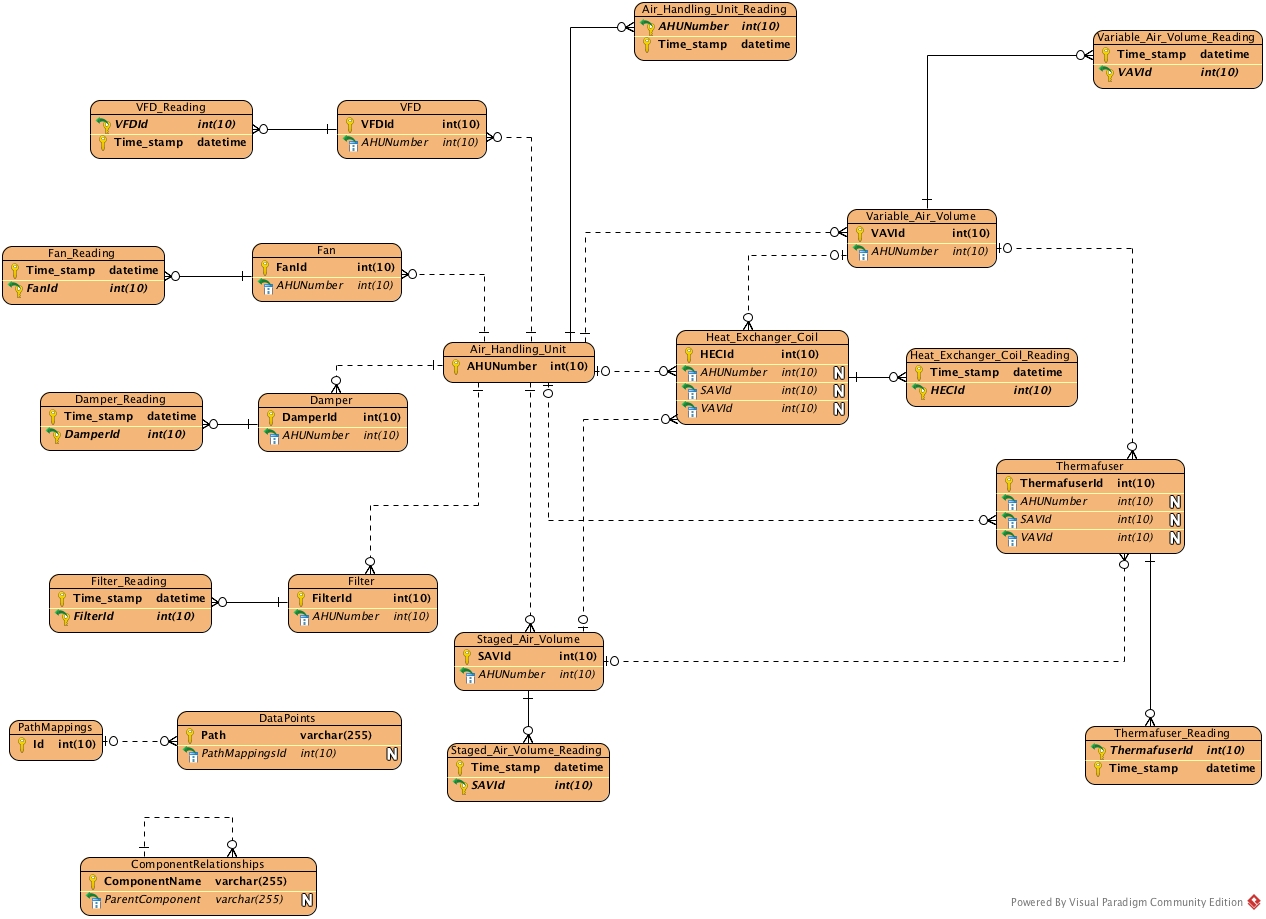
\includegraphics[width=150mm, height=100mm]{resources/HVAC_SE2_Names.jpg}
  	\caption{Proposed Database Design}
  	%\captionof{figure}{A figure}
 	\label{fig:databaseDesign}
\end{figure}

To save space only the tables, its primary and foreign keys and the relationships between tables are shown in Figure \ref{fig:databaseDesign}. The specific attributes for each table can be found in the Appendix \ref{section:appendixA}. Next, a discussion of the structure of the database is presented. 

As can be observed in the diagram presented in Figure \ref{fig:databaseDesign}, the central element is the \gls{ahu} table. An \gls{ahu} can supply conditioned air to many \glspl{vav}/\glspl{sav} while a \gls{vav}/\gls{sav} can only be supplied air by a single \gls{ahu} (with one exception in the case of the SE 2 \gls{hvac} which will be addressed further), this relationship is modeled in the database as a one-to-many relationship between the \gls{ahu} table and the \glspl{vav}/\glspl{sav} tables.

Moving downwards in the hierarchy of the \gls{hvac} network we find \glspl{vav}/\glspl{sav}, this components are represented by its own tabled in the database. Each \gls{vav}/\gls{sav} can supply air to a number of thermafusers in the last level of the \gls{hvac} hierarchy, nevertheless a thermafuser can only be supplied air by a single \gls{vav}/\gls{sav}, once again, this represents a one-to-many relationship between the \glspl{vav}/\glspl{sav} tables and the thermafuser table.

As stated earlier, each one of the major components in the \gls{hvac} system (\glspl{ahu}, \glspl{vav}, \glspl{sav}) may be made up of some more basic components. In general, any of the major components can contain a number of fans, dampers, cooling and heating coils (generalized here as heat exchanger coils), filters and VFDs, each of these components is represented in the database by its own table. Notice here, that while a particular major component can contain many of these components a particular instance of such components can only belong to one and only one \gls{ahu}, this is again reflected as a one-to-many relationship between the major and the minor components in the database.

Finally, each one of the components of the system (major and minor) have a number of sensors that provide readings and measurements of certain variables pertinent to each device. For each device, its own readings are represented as a table (with the prefix ``Reading'' on the name of the table) where a device may have many reading but a particular set of readings can belong to only one component, once again, this is represented as a one-to-many relationship between the component and its readings in the database. For a  full description of the variables pertinent to each component please refer to Appendix \ref{section:appendixA}.

This database design not only allows for a more reliable and efficient storage of the raw data, but also will help make the fault localization more accurate, since once a fault is detected by analyzing the data, its location can be accurately given by means of the primary keys of each table and the relationships among tables.
